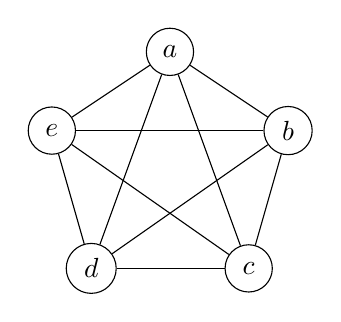
\begin{tikzpicture}
\node [circle, minimum height=0.6cm, draw] (v1) at (0,0) {$a$};
\node [circle, minimum height=0.6cm, draw] (v2) at (1.5,-1) {$b$};
\node [circle, minimum height=0.6cm, draw] (v3) at (1,-2.75) {$c$};
\node [circle, minimum height=0.6cm, draw] (v4) at (-1,-2.75) {$d$};
\node [circle, minimum height=0.6cm, draw] (v5) at (-1.5,-1) {$e$};
\draw  (v1) edge (v2);
\draw  (v2) edge (v3);
\draw  (v3) edge (v4);
\draw  (v4) edge (v5);
\draw  (v5) edge (v1);
\draw  (v1) edge (v3);
\draw  (v3) edge (v5);
\draw  (v5) edge (v2);
\draw  (v2) edge (v4);
\draw  (v4) edge (v1);
\end{tikzpicture}